\chapter{Referencial Teórico}
\label{chap:ref}

Neste capítulo são apresentados os conceitos base para a realização deste trabalho. As seções a seguir tratam sobre Interação Humano-Computador, Personas e Jogos. Por fim, são apresentados os trabalhos relacionados ao tema deste projeto.

\section{Interação Humano-Computador}

Nesta seção estão descritos os tópicos que envolvem IHC relacionados a este trabalho. Primeiramente é apresentada na subseção \ref{sub:visao_ihc} sobre a Visão de  Desenvolvimento de Sistemas em IHC; depois o seu Objeto de Estudo, na subseção \ref{sub:obj}; seguido por seu Processo de Design, subseção \ref{sub:process_ihc}, e seus Benefícios, subseção \ref{sub:quali}. No discorrer da seção são apresentados como o tema desse projeto e a técnica de Personas, se relaciona com IHC.

A disciplina de Interação Humano-Computador está voltada para o projeto, implementação e avaliação de sistemas computacionais interativos usados por seres humanos, assim como também contempla os fenômenos relacionados a esse uso \cite{hewett1992}. Para conhecer melhor os fenômenos envolvidos no uso destes sistemas, IHC acaba por se beneficiar de conhecimentos e métodos de outras áreas fora da Computação, como é o caso da Psicologia, Sociologia e Antropologia. Estas contribuem para que seja possível adquirir conhecimento sobre a cultura, sobre os usuários, sobre seus comportamentos, suas atividades, sejam elas individuais ou em grupo e entre outros elementos \cite[p. 2, 12]{barbosa_silva}.% IHC - pag 2, 12

\subsection{Visão de Desenvolvimento de Sistemas em IHC}
\label{sub:visao_ihc}
Existem diferentes visões sobre o desenvolvimento de sistemas computacionais. \citeonline[p. 7]{barbosa_silva} pontuam as seguintes visões sobre um sistema interativo: a dos desenvolvedores, que focam nas funcionalidades, aquilo que o software de fato permite ser feito; a visão do cliente responsável pela aquisição do software, que é aquilo que ele deseja que o software deva fazer; e a visão do usuário, que está relacionada ao impacto do software em seu cotidiano. A identificação das diferentes partes envolvidas e a definição dos seus interesses e pontos de vista são importantes, porém difíceis de conciliar no desenvolvimento de um software, acabando por gerar dificuldades na criação de sistemas que promovam essa interação entre ser humano e computadores. % IHC - pag 7

\citeonline[p. 8, 9]{barbosa_silva} ainda afirmam que as diversas áreas de conhecimento possuem perspectivas distintas sobre esse problema, porém a área de Interação Humano-Computador está interessada na qualidade e no impacto de uso desses sistemas na vida dos usuários. Para se desenvolver um sistema interativo adequado a um público-alvo, a área de IHC dispõem de uma abordagem de processo de design no qual:

\begin{itemize}
    \item inicia-se investigando e analisando as partes envolvidas, seus interesses, objetivos, atividades, responsabilidades, motivações, os artefatos utilizados, o domínio, o contexto de uso, dentre outros elementos;
    \item depois o projeto segue com a definição das oportunidades de intervenção onde se poderá aplicar uma solução;
    \item na sequência, vem a definição da forma que essa intervenção tomará como interface para o usuário; e
    \item finalmente, é definido as características de um sistema viável dentro dessa intervenção.
\end{itemize}    %IHC pag 8-9

De forma sucinta, a visão de IHC em relação ao desenvolvimento de sistema computacionais interativos prioriza o usuário. A partir dessa visão, a área de IHC busca estudar os elementos que envolvem a interação das pessoas e os sistemas computacionais.

\subsection{Objeto de estudo em IHC}
\label{sub:obj}
Os elementos que IHC aborda podem ser chamados de objetos de estudo. Nesta subseção estão descritos os conceitos destes objetos e suas classificações. 

De acordo com \citeonline{hewett1992}, citado por \citeonline[p. 10-12]{barbosa_silva}, os objetos de estudo de IHC podem ser agrupados em cinco tópicos inter-relacionados: %IHC pag 10-12

\begin{itemize}
    \item \textbf{Natureza da interação:} investiga o que acontece enquanto pessoas utilizam os sistemas interativos, buscando descrever, explicar e prever fenômenos e consequências do seu uso para com as pessoas;

    \item \textbf{Contexto de uso:} busca conhecer como determinada cultura, sociedade e organização conseguem influenciar na interação das pessoas com os sistemas. Este conhecimento é bastante importante pois o contexto do desenvolvedor e do usuário costumam ser diferentes;

    \item \textbf{Características humanas:} elas merecem atenção, pois influenciam na forma das pessoas interagirem com os sistemas computacionais. A capacidade cognitiva, a forma com que a pessoa se comunica e interage com outras pessoas, as características físicas motoras e sensoriais de cada pessoa impactam na forma que elas irão usar os sistemas;

    \item \textbf{Arquitetura e a interface do sistema:} busca abordar a construção de dispositivos e sistemas interativos de forma que favoreçam a experiência do usuário; e

    \item \textbf{Processo de Design:} o processo influencia a qualidade do produto final. Sendo assim, é importante conhecer as abordagens de design, métodos, técnicas e ferramentas para a construção e avaliação de interfaces em IHC. 
\end{itemize}

A partir do estudo destes objetos são desenvolvidas técnicas, métodos, ferramentas, frameworks, padrões e entre outros produtos que podem ser usados no desenvolvimento de sistemas interativos.

\subsection{Processo de Design em IHC}
\label{sub:process_ihc}
Nesta subseção é apresentado o conceito base do Processo de Design, um dos objetos de estudo de IHC. Entender o processo de design é importante, até mesmo, para apoiar o estudo dos demais objetos abordados pela área de Interação Humano-Computador, norteando em que momento do design a aplicação prática desses estudos podem ser utilizadas.

\citeonline{lawson2006} apresenta que o processo de design em IHC aborda as seguintes atividades basicamente: a análise da situação corrente, que compete a identificação do problema e elementos que o envolve; a síntese de uma intervenção, na qual é elaborada a proposta de solução; e a avaliação da intervenção, que trata da viabilidade da solução. 

Cada processo de design modela essas atividades base de forma diferente, dependendo dos princípios que autor do processo quer enfatizar. Sendo assim as atividades podem variar quanto à sua forma de execução, sua sequência, sua repetição, seus motivos e os artefatos gerados \cite[p. 92, 99]{barbosa_silva}. % IHC - pg 92, 99

Porém uma característica fundamental dos processo de design em IHC é a execução iterativa de suas atividades. Isso faz com que seja possível ocorrer sucessivas modificações e melhorias na análise da situação e na síntese de intervenção a partir da avaliação dessas atividades \cite{barbosa_silva}. Para \citeonline[p. 100]{lawson2006} essas atividades não necessitam de uma sequência de transição estrita. Segundo ele é possível começar o processo de design em qualquer atividade e realizar uma transição pra qualquer outra atividade sempre que for necessário, como é mostrado na Figura \ref{Fig:design_process.png}. %pag 100

\begin{figure}[htbp]
	\centering
		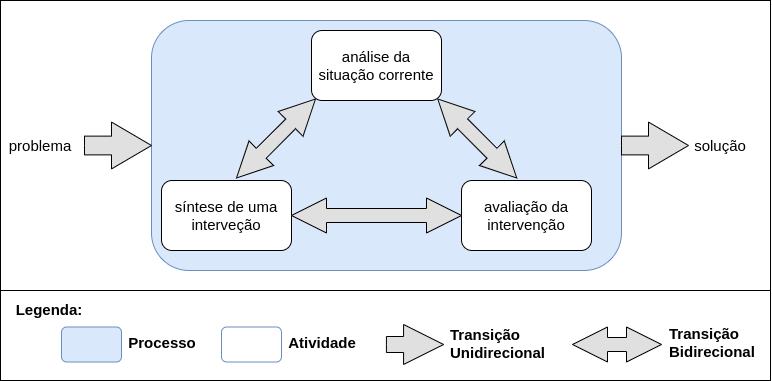
\includegraphics[keepaspectratio=true,scale=0.5]{figuras/process_design.png}
	\caption{Processo de design genérico - adaptado de \citeonline{lawson2006}.}
	\label{Fig:design_process.png}
\end{figure}

O que importa é partir de um problema (as necessidades e oportunidades de melhoria na situação atual), realizar o processo de design (atividades de análise, síntese e avaliação) e no fim chegar a uma solução (uma proposta de intervenção). Cabe ao designer decidir qual será a primeira atividade a ser executada e as transições a serem feitas \cite[p. 100]{lawson2006}. %pag 100

\subsection{Qualidade em IHC}
\label{sub:quali}
Para finalizar a seção, é apresentado nesta subseção os benefícios de se adotar a visão de desenvolvimento, conceitos e elementos do campo de IHC.

A qualidade de uso trata do estudo daquilo que envolve a interação entre seres humanos e sistemas computacionais permite ao profissional responsável por desenvolver essas tecnologias, a possibilidade de construí-las, melhorá-las e inseri-las na vida das pessoas sempre buscando uma boa experiência de uso. Isto pode ser traduzido na busca pela qualidade de uso desses sistemas interativos, que é visão da área de IHC \cite[p. 13, 14]{barbosa_silva}.%IHC pag 13-14

\citeonline{barbosa_silva} descrevem como critérios de qualidade na interação dos usuários com as interfaces: a usabilidade; a experiência do usuário; a acessibilidade; e a comunicabilidade. \citeonline{Petri_Wangenheim_2019} focaram em trabalhar com a qualidade de jogos educacionais por meio do modelo MEEGA+, que visa os fatores de usabilidade e experiência do jogador a partir da perspectiva do aluno. 

\citeonline{Petri_Wangenheim_2019} definem usabilidade como \textit{"o grau em que um produto (jogo educacional) pode ser usado por usuários específicos (alunos) para atingir objetivos específicos com eficácia e eficiência em um contexto de uso especificado (educação em computação), sendo composto pelas seguintes dimensões: estética, capacidade de aprendizagem, operabilidade e acessibilidade"}. E definem a experiência do jogador como \textit{"um fator de qualidade que abrange um envolvimento profundo do aluno na tarefa de jogo, incluindo sua percepção de aprendizagem, sentimentos, prazeres e interações com o jogo, ambiente e outros jogadores, sendo composta pelas seguintes dimensões: atenção focada, diversão, desafio, interação social, confiança, relevância, satisfação e aprendizagem percebida"}. A tabela com os fatores dimensões e definição do modelo MEEGA+ pode ser encontrada no Anexo \ref{an:meega}. % citação direta - MEEGA+ pg 5

Segundo \citeonline[p. 13, 14, 28]{barbosa_silva} trabalhar bem esses critérios contribui de forma benéfica para com o produto e consequentemente para com o usuário. São estes os benefícios: %IHC pag 13-14, 28

\begin{itemize}
    \item aumentar a produtividade dos usuários, pois com uma interação eficiente, os usuários poderão alcançar seus objetivos utilizando o sistema desenvolvido com esse foco;

    \item reduzir o número e a gravidade dos erros cometidos pelos usuários, pois os usuários poderão ter mais clareza em suas ações no sistema prevendo e evitando resultados indesejados;

    \item reduzir o custo de treinamento, pois com um design intuitivo o usuário poderá aprender por si só como interagir com o sistema;

    \item reduzir o custo de suporte técnico, pois caso ocorra algum erro o próprio sistema irá direcionar o usuário para resolve-lo; e

    \item e aumentar as vendas e a fidelidade do cliente, pois com a satisfação do usuário há um aumento da confiança e aquisição de novas versões e outros sistemas.
\end{itemize}

Na sequência é apresentada a técnica de personas. Esta se enquadra na visão de IHC no quesito de buscar abstrair melhor os desejos do usuário sobre o uso de um sistema interativo. 

\section{Personas}

Nesta seção é apresentada a Técnica de Persona. Aqui é abrangido seu contexto de aplicação, sua definição, e como são classificadas.

\subsection{Contexto de Aplicação}

Nesta subseção é introduzido onde a técnica de persona se enquadra no processo de design de interface e por qual objeto de estudo de IHC ela está ligada. Também é relatado qual o contexto e problema a técnica busca atacar.

Como definido por \citeonline{lawson2006} nos processos de design de sistemas interativos, a atividade de análise da situação contempla a identificação, organização, refinamento e estudo dos elementos do contexto de uso do sistema e das características do usuário \cite{hewett1992}. Levando isso em conta, quando se tratam de projetos com a visão de IHC, que é centrada no usuário, é importante para o profissional que desenvolve a interface do sistema compreender bem essa etapa para que seja desenvolvido um produto que satisfaça a necessidade de seu público-alvo \cite{barbosa_silva}. % compilado de um bocado de trechos

Para criar um produto que satisfaça um público heterogêneo, a primeira vista, a lógica pode dar a direção de se criar uma solução mais abrangente possível, porém para \citeonline{cooper99} a melhor estratégia é projetar esse produto para atender indivíduos específicos com necessidades específicas. \citeonline{cooper07} diz que estender a abrangência do produto com o objetivo de contemplar muitos usuários acaba colocando outros obstáculos para usuários que já haviam sido contemplados. \citeonline{cooper07} afirmam que a chave para resolver esse problema é identificar indivíduos para o projeto, cujas necessidades representam um público maior e depois de definidos, priorizá-los de acordo com sua importância. 

E é neste contexto que são aplicadas as personas. \citeonline[p. 77]{cooper07} veem as personas como uma ferramenta que torna claros os objetivos dos usuários, definindo o que o produto deve ou não fazer. \citeonline{barbosa_silva} dizem que as personas auxiliam o designer a justificar suas decisões no projeto. Assim, ao projetar o design para um conjunto pequeno de personas aumenta as chances da interface atender as expectativas e satisfazer o público-alvo. % About face 3 - pg 77

Segundo \citeonline{barbosa_silva} uma prática adotada pelas equipes de design é reconhecer as personas como integrantes do time. Adotando essa abordagem é preciso o time deixar o termo "usuário" de lado e constantemente se referenciar às personas por seus nomes. \citeonline{cooper99} vai mais a fundo e diz que quando a equipe consegue se colocar no lugar da persona, incorporando suas características, ao participar do processo de design é possível ter um melhor \textit{feedback} se o design está sendo bem sucedido ou não. 

\subsection{Definição de Persona}

Nesta subseção é relatado o que é uma persona e como defini-las. Elas são personagens fictícias e hipotéticas, que representam e descrevem um grupo de usuários reais e que são definidas principalmente por seus objetivos, definidas e refinada durante a investigação dos usuários \cite[p. 176]{barbosa_silva, cooper07, pruitt, cooper99}. % IHC pg 176

Elas são definidas a partir de dados de campo, onde são identificadas diferentes características dos usuários. Estas podem variar desde aspectos demográficos como sexo, faixa etária e classe social até perfis comportamentais \cite[p. 81]{Vianna_2014}. Como é definido por \citeonline{Courage_Baxter_2005}, citado por \cite[p. 177]{barbosa_silva} uma persona possue as seguintes características: %Design Things pg 81 / IHC pg 177

\begin{itemize}
    \item \textbf{identidade:} para que exista mais realismo para a persona, é impostante que ela tenha um nome, idade, outros dados demográficos e uma foto;

    \item \textbf{status:} define o tipo das personas, priorizando-as em primária, secundária, suplementar, cliente, servida ou anti-persona;

    \item \textbf{objetivos:} condição final a ser atingida, que nesse caso não se restringe ao produto, podendo ser um objetivo pessoal, corporativo, prático etc;

    \item \textbf{habilidades:} especialidades, educação, treinamento e competências que podem não ser necessariamente relacionadas ao produto; 

    \item \textbf{tarefas:} aquilo que a persona executa, sendo elas básicas ou críticas, podendo ser classificadas quanto a sua frequência, importância e duração;
    
    \item \textbf{relacionamentos:} entender com quem a persona interage, pois isso ajuda a identificar outras partes envolvidas;
    
    \item \textbf{requisitos:} aquilo que as personas precisam, suas necessidades; e
    
    \item \textbf{expectativas:} o que a persona espera do produto em relação ao seu funcionamento, aquilo que o produto gera enquanto a persona interage com ele.
\end{itemize}

Mesmo as personas sendo fictícias, elas são elaboradas com rigor e detalhes para representar os usuários reais. A partir de um processo de investigação das características dos usuários e descrição de seu perfil são elaboradas as personas. Sendo assim, a eficiência dessa ferramenta de design está atrelada ao quão próxima a persona se encontra de uma pessoa real e o quanto ela representa o seu público-alvo \cite[p. 177]{barbosa_silva}. % IHC pg 177

\subsection{Elenco das Personas}

Esta subseção trata do elenco de personas e a prioridade de cada uma das personas elaboradas. O elenco de personas de um projeto conta com pelo menos três personas distintas como descrito por \citeonline{Courage_Baxter_2005} e \citeauthor{usability2020}, e são seis os seus tipos, conforme foi definido por \citeonline{cooper07}.

O elenco de persona é caracterizado por conter ao menos uma persona por papel de usuário e ao menos uma delas deve ser a persona primária \cite{barbosa_silva}. Elas são classificadas quanto a sua prioridade em relação ao foco do design da interface do sistema desenvolvido. São os tipos de personas segundo é descrito por \citeonline{cooper07}:

\begin{itemize}
    \item Persona Primária: esta representa o principal alvo do design. Ela é que tem de ser satisfeita pela interface projetada;
    
    \item Persona Secundária: esta é satisfeita com a interface projetada para a persona primária, porém a persona secundária necessita de adicionais específicas que podem ser acrescentadas ao design sem prejudicar aquilo que foi projetado para servir à persona primária;
    
    \item Persona Suplementar: ela é uma combinação das personas  primárias e secundárias. Suas necessidades são completamente representadas por essa combinação de personas;
    
    \item Persona do Cliente: esta persona busca atender às necessidades dos clientes, que não necessariamente são dos usuários finais do sistema;
    
    \item Persona Servida: este tipo de persona é diferente do tipos de persona já discutidos. Ela não é um usuário do produto; contudo, eles são diretamente afetados pelo uso do produto; e
    
    \item Persona Negativa: chamada também de anti-persona, esta persona é usada para comunicar às partes interessadas e demais \textit{stakeholders} que existem tipos específicos de usuários para os quais o produto não foi projetado. 
\end{itemize}

\section{Jogos}

Nesta seção são apresentados a definição de jogos e jogos sérios encontrados na literatura. Também é abordado sobre o ensino e aprendizagem usando jogos.

Segundo \citeonline{Fullerton_2008} jogo é \textit{"um sistema fechado e formal que envolve os jogadores em conflitos estruturados e resolve sua incerteza em um resultado desigual."} Quando é dito que jogos são sistemas fechados, trata-se dos limites. Um jogo possui regras, contexto e demais elementos restritos a ele que são separados do mundo real e suas regras, contexto e entre outros elementos. 

Os jogos são formais, ou seja, são estruturados por elementos formais que se relacionam entre si, que podem se diversificar dependendo do tipo de jogo. Juntamente com esse elementos formais os jogos contemplam elementos dramáticos, que assim estruturam um conflito que envolve um ou mais jogadores. E por fim os jogos envolvem incerteza quanto aos seus resultados desiguais, em que, enquanto não há resultado existe a incerteza e quando há resultado, este é desigual sempre havendo vencedores e/ou derrotados, seja entre jogadores ou entre um jogador e algum desafio \cite{Fullerton_2008}.

Uma outra definição mais prática abordada por \cite{McGonigal_Rieche_2012} é que os jogos compartilham de quatro características que os definem: meta, regras, sistema de \textit{feedback} e participação voluntária. Demais elementos formais e dramáticos como interatividade, gráficos, narrativa, recompensas, competitividade, personagens, gênero dentre outros, são características comuns a muitos jogos, mas não definidoras \cite{Vianna_Vianna_Medina_Tanaka_Krug_2013}.

A academia veio pesquisando ao longo do tempo formas alternativas e instigadoras para motivar a aprendizagem dos alunos e um desses meios são os jogos. No geral, foi observado nos jogos a sua capacidade de atrair e motivar as pessoas e de gerar engajamento e dedicação na realização de tarefas \cite{Vianna_Vianna_Medina_Tanaka_Krug_2013}. Os Jogos Sérios (\textit{Serious Games}) são jogos com uma finalidade que vai além do entretenimento. No caso da educação, o uso de jogos busca tornar o processo de ensino-aprendizagem mais atrativo e proveitoso, desenvolvendo no estudante habilidades cognitivas através da prática e engajar os alunos nesse processo \cite{sommariva, queiroz, darin}.

Existem várias áreas onde o jogos são aplicados no intuito de auxiliar o ensino e aprendizagem. Uma dessa áreas é a de Interação Humano-Computador \cite{Sales2020, Sales2020UsoTDS}.

\section{Trabalhos Correlatos}
\label{sec:trab_cor}

Nesta sessão estão apresentados os estudos sobre jogos educacionais em IHC, aplicados em cursos de graduação e pós graduação. Estes trabalhos são resultado de uma Revisão Sistemática de Literatura da pesquisa de \citeonline{deSales_SousaeSilva_2020}. No estudo foram identificados seis jogos e suas características, os requisitos não funcionais e aspectos de experiência do usuário. Na sequência são apresentados brevemente estes jogos e para mais detalhes é só acessar o artigo completo \cite{deSales_SousaeSilva_2020}.

O UsabilityGame, um jogo para um jogador que simula um cenário de uma empresa de desenvolvimento de software fictíıcia (Booble Corporate), onde o jogador encarna o papel de engenheiro de usabilidade e participa de um processo de desenvolvimento relacionados a design de interação \cite{sommariva}.

O UsabiliCity, por meio de analogias com problemas numa cidade, traz o estudante para o papel de um inspetor (representado por um menino com uma lupa), que deve ajudar a população da cidade (UsabiliCity) a identificar e solucionar os seus problemas fazendo uso das dez Heurísticas de Nielsen e sua técnica de Avaliação Heurística \cite{ferreira2014a, ferreira2014b}.

No jogo MACteaching, o estudante é inserido na história em que numa cidade, Interacionópolis, a bruxa Ruptura insere várias rupturas de interação nas interfaces dos sistemas da cidade. O objetivo é identificar, para cada ruptura, a etiqueta que expressa um problema de comunicabilidade seguindo o Modelo de Avaliação de Comunicabilidade (MAC)\cite{brito, queiroz}.  
O jogo de cartas G4H (Game for Heuristic Evaluation), visa aumentar o envolvimento de diferentes avaliadores num processo de avaliação baseado-se na Avaliação Heurística \cite{juca2017}.

O jogo de cartas G4NHE (Game for aNyHeuristic Evaluation), uma generalização do G4H, tem como proposta o aumento do envolvimento  entre  diferentes  avaliadores  num  processo  de    Avaliação Heurística aplicada às diferentes Heuríısticas de usabilidade \cite{deSousa2019}.

O jogo de cartas e tabuleiro Desafio de Design Goople, que objetiva apoiar o ensino do design de interação e conceitos básicos sobre o processo de design de interfaces \cite{darin}.

Com base nesta RSL, pode-se perceber a existência de jogos educacionais em IHC voltados para auxiliar o processo de ensino e aprendizagem sobre avaliação heurística, princípios de usabilidade, aspectos teóricos das fases do processo de design de interface e também uma simulação prática desses aspectos. Tendo isso em vista, encontrou-se mais um reforço que apoie o desenvolvimento de um jogo em IHC com uma temática diferente.

